The Interprocedural Field Sensitive Shape Analysis is implemented as a plugin which adds this analysis as one of the passes in GCC.
In the first section a few details about GCC internals are given. Then in the last three sections testing strategy, optimizations and results 
are discussed.

\section{GCC Internals}

\textbf{PLUGINS:}\ Plugin's make the developer add new features to the compiler without modifying the compiler itself.
It is a way of adding, removing and maintaining modules independently. This feature is available from gcc 4.5 and later versions only.
Before we discuss plugins, we present some basic information about GCC architecture. 

The GCC architecture has many passes in it each being either
a GIMPLE, IPA (Interprocedural Analysis) or RTL(Register Transfer Language) pass. So whenever we want to add a pass in GCC we need to talk to the 
pass manager which is located in three files 'passes.c', 'tree-optimize.c' and 'tree-pass.h' and in some way these files need to be modified. And once 
modified we need to build the entire GCC so as to get the pass included in GCC.

But as GCC code base is a very large so it would take lot of time to build each time we change our pass source code. At this 
point plugins make our life easy.
Using plugins we will be able to write a shared object (.so) file that can be loaded into GCC and attached to various stages of
compilation without touching the GCC source code, hence no need of compiling gcc source every time. \\ \\
\textbf{TREE:}\ Tree is the central data structure used by GCC in its internal representation. It can point to a lot of types and to know the particular
type we need to refer TREE\_CODE macro. Each Tree usually have two fields named TREE\_CHAIN and TREE\_TYPE.
While TREE\_CHAIN contains the pointer to next tree (where all the Tree's are arranged in a singly linked list fashion), TREE\_TYPE has information 
about Type or declaration.

\textbf{GIMPLE:} \ Our analysis is performed on the GIMPLE statements which are generated by gcc in its compilation process.
Whenever GCC receives a source file say C source code, the GCC frontend invokes the gimplifier for each function which converts the source code to 
GIMPLE, which is understood by language independent parts of the compiler.
Its actually a 3-address representation with at max one load/store per statement, with memory loads only in RHS and store in LHS of assignment statements.

All the GIMPLE statements that are present in a basic block are in the form of a doubly linked list. Any manipulation to be done on them
require iterators provided by GCC. Our analysis is written as an Inter procedural gcc plugin which operates on the callgraph. In our analysis we 
need to identify whether a particular statement is one among the basic pointer statements.
The example code in Program ~\ref{gimpleAssignment} gives us the details about identifying heap manipulation statement {\tt p = NULL;}. Similarly the other
types of pointer statements are also identified.

\begin{figure}
\begin{lstlisting}[caption={Code to identify pointer statement p = NULL} ,label=gimpleAssignment]
 
if(is_gimple_assign(stmt))
{
    tree lhsop=gimple_tree_lhs(stmt)
    tree rhsop1=gimple_tree_rhs1(stmt);
    tree rhsop1 = gimple_assign_rhs1 (stmt);

    int  lhsCode=TREE_CODE(lhsop);
    int  rhsCode=TREE_CODE(rhsop1);

    if((lhsCode==VAR_DECL || lhsCode==PARM_DECL) && rhsCode1==INTEGER_CST)
      {
	  if(POINTER_TYPE_P(TREE_TYPE(lhsop)) && 
		(TREE_CODE(TREE_TYPE(TREE_TYPE(lhsop))) == RECORD_TYPE))
	    return TRUE;
	  
	  return FALSE;
      }   
}

\end{lstlisting}
\end{figure}

\section{Implementation}
Lets have an overview of the plugin that inserts this analysis as a pass in GCC.
First it finds out what are the heap pointers present in the input program and then accumulates 
information about its properties like its type, to which struct or union its pointing, fields present in that data type etc.
Along with heap pointers, field pointers are also identified whose properties are stored. Field pointers are 
pointers to some struct or union but is also a member variable of some struct or union.
After this we parse all the GIMPLE statements one by one and check if it is one of the basic statements.
If the identified statement is a pointer assignment statement a new dummy statement (as discussed in Chapter~\ref{Enhancements}) is inserted before it.
Also we modify the Control flow graph by inserting callblocks and return blocks if necessary.
Since the data flow values may change for any of those statements, whenever any of those is encountered GEN and KILL are evaluated, followed by 
calculation of OUT from IN, GEN and KILL in the usual way.i.e  
\[
OUT = GEN \cup (IN - KILL)
\]
All the equations for GEN and KILL of each statement are mentioned in Fig.~\ref{fig:Modified Data Flow Equations}. As we have modified 
the Control flow graph initially before returning we restore the CFG to its original form. The below pseudo code gives the flow of the implementation.
\begin{figure}[h]
\begin{lstlisting}
begin
  gatherHeapandFieldPointers();
  preprocess_CFG();  
  shapeAnalysis();
  restore_CFG();
end
\end{lstlisting}
\end{figure}
In the function shapeAnalysis the actual identification of shape is done. This is implemented as a 
worklist based interprocedural analysis, so whenever the worklist goes empty the analysis is stopped.

Now we will discuss the data structures used to 
contain the data flow values. The Direction Matrix and Interference Matrix  are represented as an adjacency matrix with each cell 
being a pointer to nested structures.
These were designed in such a way to handle all the possible values that can be present in each cell.
The boolean equations are represented as character strings. This representation leads to huge memory consumption as we need to store them at
each program point.
Also the size of equation grows with the program, thus taking more time to evaluate. We have tried to resolve these problems to some extent by 
performing some memory and time optimizations.Next we discuss some memory and time optimizations performed.
\subsection{Storing of boolean equations}
Consider the control flow graph in Fig:~\ref{CFG_1}(a) which represents a program containing if-else statements. 
\begin{eqnarray*}
 {IN}_{eq}(S1) &=& {OUT}_{eq}(bb0) \\
 {IN}_{eq}(S2) &=& {OUT}_{eq}(bb0) \\
{OUT}_{eq}(S1) &=& {GEN}_{eq}(S1) \cup ( {IN}_{eq}(S1) - {KILL}_{eq}(S1)  ) \\
{OUT}_{eq}(S2)  &=& {GEN}_{eq}(S2) \cup ( {IN}_{eq}(S2) - {KILL}_{eq}(S2)  ) \\
{OUT}_{eq}(bb1) &=& {OUT}_{eq}(S1) \\
{OUT}_{eq}(bb2) &=& {OUT}_{eq}(S2) \\
{IN}_{eq}(bb3) &=& {OUT}_{eq}(bb1) \cup {OUT}_{eq}(bb2)
\end{eqnarray*}

Both ${OUT}_{eq}(bb1)$ and ${OUT}_{eq}(bb2)$ have a copy of ${OUT}_{eq}(bb0)$ in them, so ${IN}_{eq}(bb3)$  also has two copies of it.
This may seem very little amount of redundancy but actually for a large program this would become a very big problem.

Instead of storing two copies of the same equation we can save memory by storing the equation at some place and just
store pointers to that equation. So now both ${OUT}_{eq}(S1)$ and ${OUT}_{eq}(S2)$ will not have the
copies of ${OUT}_{eq}(bb0)$ in it  but just the pointers to them.
For this optimization to occur we should keep all the data flow boolean equations at each statement.
But just doing this change isn't enough. Lets look at  Fig:~\ref{CFG_1}(b) for the issue with this. This figure shows us a small part
of CFG of a program containing while loop.

First time we process {\tt S1}, {\tt S2},as discussed just above, we will be keeping their corresponding boolean equations. There is a very good 
chance that 
boolean equation at {\tt S2} has a pointer to the boolean equation at {\tt S1}. Now this information is passed to bb1 which gets passed to S1 itself.
As we are storing the equation again we will be overwriting the already present boolean equations with the current incoming equations, causing loss of information. The similar case can occur in recursive programs too. In order to avoid this we have to keep versions
of this equations, and keep track of the version number when pointing to boolean equations.
This change significantly reduces the amount of memory consumption.

\begin{figure}[h]
\begin{tabular}{cc}
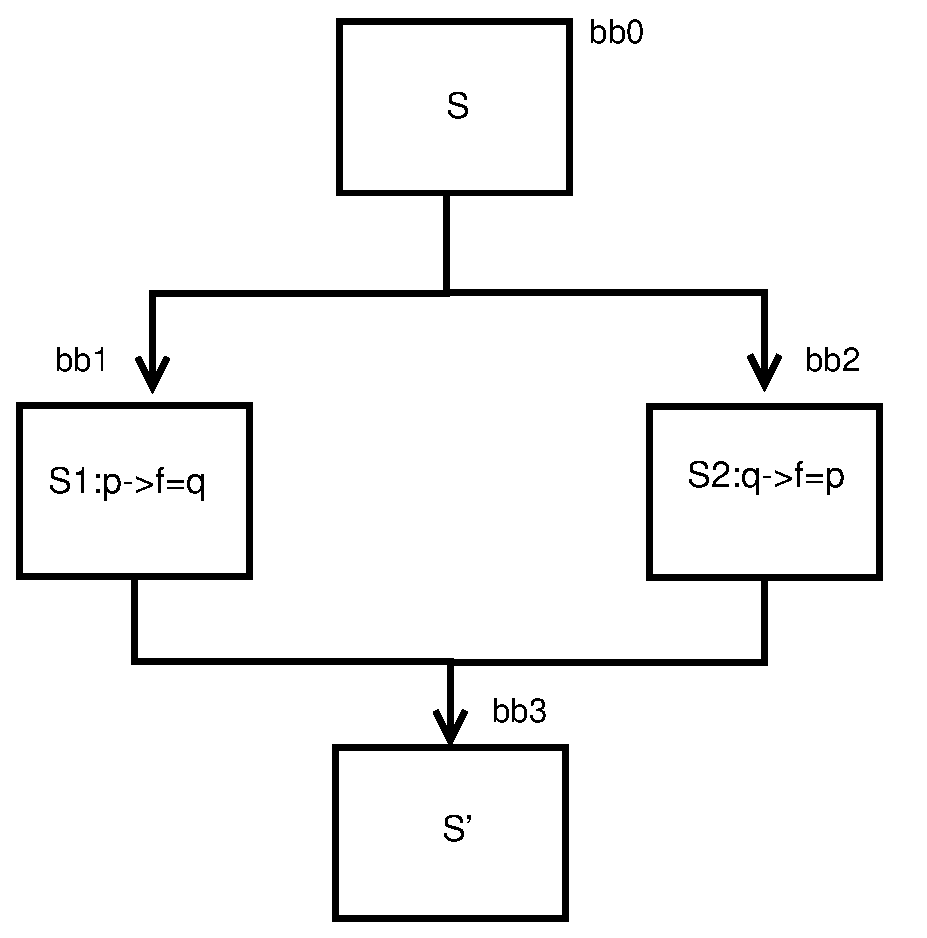
\includegraphics[scale=.4]{diagrams/Enhancements_d1.eps} & 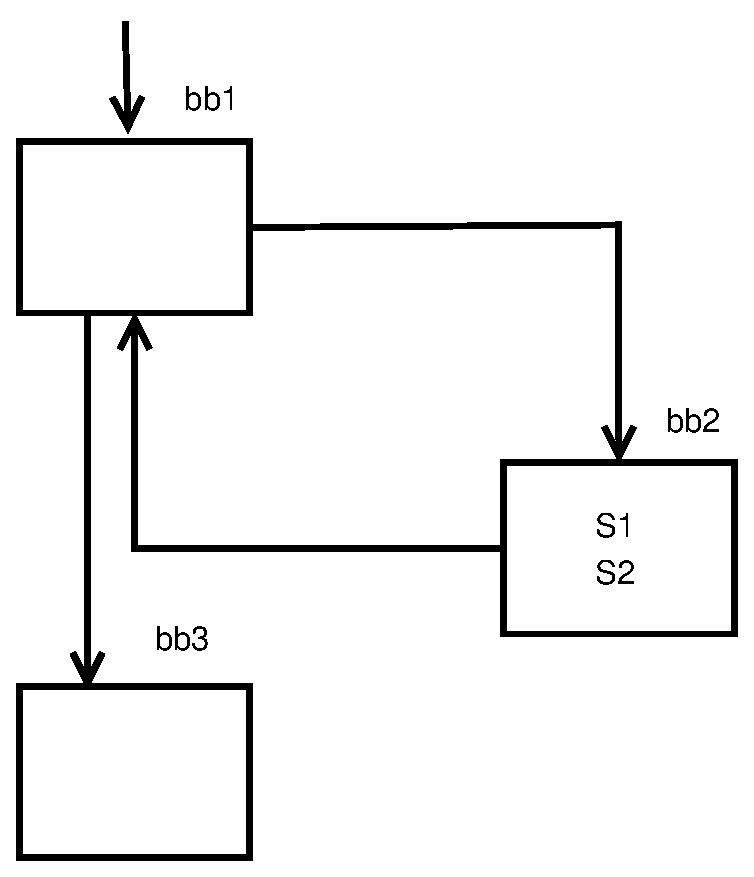
\includegraphics[scale=.4]{diagrams/Enhancements_d2.eps} \\
\footnotesize (a) & \footnotesize (b) 
\end{tabular}
\caption{CFG example}\label{CFG_1}
\end{figure}    


\subsection{Time optimization}
%We have just seen in the above subsection that there may be repetitions of
%terms in the boolean equaitons when conditional, looping or recursion is present in programs. Then why not remove the redundant terms in those 
%equations.Again here the time
%consumption is a problem,because manipulating strings as we know is a very costly operation.

% Because of this time constraint we haven't removed the redundant terms,
% but to reduce the computatuion time we have been hashing the results of these repeated terms.
Initially when we just stored the  boolean equation as it is and for that the  time taken for the analysis 
of merge\_recur to complete was \textbf{4 hrs}. But later we realized that, during the evaluation of boolean equation we are converting it to postfix, 
it is effective to store the postfix equation itself instead of infix. After this change the time for the analysis 
of merge\_recur reduced to \textbf{2 hrs}.

We have just seen in the above subsection that there may be repetitions of
terms in the boolean equations when conditional, looping or recursion is present in programs. Careful analysis of the equation for some sample programs 
made us notice that the time taken to evaluate these repeated terms can be cut down if we store their results in  some hash table and reuse 
whenever repetition occurs. This has reduced the time taken drastically, and the analysis of merge\_recur comes down to \textbf{35 seconds}.

\section{Testing Strategy}
We all know how important testing is in order to determine whether we are meeting our required results. In our analysis with the source code 
spanning close to 12000 LOC and a vast range of possible testcases, an efficient testing strategy is a must. 
  
We have written a script that could generate us many unit testcases depending on the number of statements that we want to have in our test case.
A sample template of how our testcase looks is presented in Program ~\ref{template}

\begin{figure}
\begin{lstlisting}[caption={Unit Testcase Template} ,label=template]
 
#include <stdlib.h>
int main()
{
	 typedef struct _node node;
	 struct _node {
		 node* f;
		 node* g;
	};

	 node* p = (node*)malloc(sizeof(node));
	 node* q = (node*)malloc(sizeof(node));

	/* HEAP MANIPULATION STARTS */
	.......
	.......
	/* HEAP MANIPULATION ENDS   */

}
\end{lstlisting}
\end{figure}
     
It is at those dotted lines that our pointer statements will be inserted. You could see in the template that the number of heap pointers are 2 and 
number of field pointer are 2.
With these properties the number of possibilities for each statement is 42, some of the possible statements are $\p \rightarrow \f =  \q$,$\p \rightarrow \g =  \q \rightarrow \f$, $\p \rightarrow \f = malloc() $, $\p = NULL$ and so on. If we increase the number of heap pointers or field pointers the 
possibilities for each statement would further increase.
The number of test cases generated for different number of statements is given in the Table.~\ref{TestCaseCount}
Once we have generated the testcases we run GHIYA's analysis and our analysis and compare the results for each. By comparison we mean comparing the shape 
of each pointer
after each GIMPLE statement.
Based on the comparison we put the test case in one of the three categories: PASS, SAFE, FAIL/ACCURATE. \\

\begin{itemize}
 \item PASS : GHIYA's analysis and our analysis gives the shape information at all statements
 \item SAFE : GHIYA's analysis is more accurate than us, .i.e for example if our analysis infers the shape as CYCLE, then Ghiya will
 infer more precise shapes like DAG or Tree.
 \item FAIL/ACCURATE : Our analysis gives less conservative shapes than GHIYA. If this happens then there could be two scenarios: 
 either we are giving accurate results or we are giving incorrect results. 
 All the testcases present in this case  are checked manually we ensure that we are not getting any fail cases.
\end{itemize}

\begin{table}
 \begin{center}
\begin{tabular}{|c|c|}
 \hline
 {\bf No Of Stmts} & {\bf TestCases Generated} \\ \hline
  1  & 42 \\ \hline
  2  & 1764 \\ \hline
  3  & 74088 \\ \hline 
\end{tabular}
\end{center}
\label{TestCaseCount}
\caption{No Of TestCases} 
\end{table}

\section{Results}
% \label{intro:community}

This section contains details about how would the Field sensitive analysis 
performs in terms of accuracy and performance when run on different benchmarks.
We also give results when this analysis is run on unit test cases. Every time we compare
the results with Ghiya method \cite{Ghiya96}. Ghiya's shape analysis is also
implemented as a GCC plugin which does context insensitive shape analysis.
First we will look at how the analysis performs on the unit test cases (about which we explained in earlier section)
and later we will show its performance on List benchmarks followed by one of the olden benchmark. The configuration of the machine used for
the generation of results are 2 GB RAM, Pentium Dual Core, 2.10Ghz. \\ \\
\textbf{Unit Test cases: }The details about these Unit Test cases are already given in the previous section.
All these test cases are compared with Ghiya's analysis.
Here  a comparison is done on how the results have varied before and after all the enhancements 
mentioned in Chapter 3 were included. They are given in the Table ~\ref{UnitRes}.

\begin{table}
 
\centering
\begin{tabular}{|c@{}|@{}c@{}|@{}c@{}|@{}c@{}|@{}c|}
 \hline
& TestCases & Pass & Safe & Accurate \\ \hline
Before \  & 
\begin{tabular}{c}
  ml-1 \\
  ml-2 \\
  ml-2-if \\
  ml-2-while \\
  ml-3
\end{tabular}
&
\begin{tabular}{c}
 42\\
 1572 \\
 1764 \\
 1108 \\
 51854
\end{tabular}
&
\begin{tabular}{c}
 0 \\
 24 \\
 0 \\
 452 \\
 6864
\end{tabular}
&
\begin{tabular}{c}
 0 \\
 168 \\
 0 \\
 204 \\
 15370
\end{tabular}
\\  \hline%----after
After & 
\begin{tabular}{c}
  ml-1 \\
  ml-2 \\
  ml-2-if \\
  ml-2-while \\
  ml-3 
\end{tabular}
&
\begin{tabular}{c}
  42\\
 1612 \\
 1764 \\
 1452 \\
 58444
\end{tabular}
&
\begin{tabular}{c}
 0\\
 0 \\
 0 \\
 0 \\
 0 
\end{tabular}
&
\begin{tabular}{c}
 0 \\
 152 \\
 0 \\
 312 \\
 16202
\end{tabular}
\\ \hline
\end{tabular}

\caption{Unit test cases results} \label{UnitRes}
\end{table}

   We have already mentioned about the script used to generate these unit test cases, these test cases can have any number of heap manipulation
statements as we desire. All those test cases with one heap manipulation are said to be ml-1, those with two as ml-2 etc.
Referring to template Program~\ref{template}, in the area where the heap manipulation statements are to be inserted, for ml-while and ml-if type test cases,  
while and if conditional statements are put. The template for these two are given below. The statement {\tt \p \ = null} was added just to find the
shape after these conditionals are executed. 

\begin{table}[h]
\centering
\begin{tabular}{ccc}
\begin{tabular}{l}
statement\_1 \\
while (condition)\{ \\
\ \ statement\_2 \\
\} \\
p = null; \\
\end{tabular}
& &

\begin{tabular}{l}
if (condition) \\
\ \ \ statement\_1 \\
else \\
\ \ \ statement\_2 \\
p = null; \\
\end{tabular}

\\ 
\footnotesize (a)ml-2-while & & \footnotesize (b)ml-2-if
\end{tabular}

\end{table}


The meaning of terms {\tt Safe},{\tt Pass},{\tt Accurate} are already explained in the previous section,but still just to reiterate.
\begin{itemize}
 \item {\tt Safe} : The shape inferred by Ghiya's analysis is more precise than that inferred by Sandeep's
 \item {\tt Accurate}: The shape inferred by Sandeep's analysis is more precise than that inferred by Ghiya's
 \item {\tt Pass} : The shape inferred is same by both the analysis.
\end{itemize}


When we look at the ml-2 results the number of {\tt Accurate} cases were more initially than there were after the enhancements. Though this was the case here we were able to
reduce the {\tt Safe} cases to 0 sacrificing some of the {\tt Accurate} cases. One such case is already mentioned in the Chapter~\ref{Enhancements}'s last part
about Information passed to successors. In ml-2-while there is a significant improvement in how the results turned out, the same can be noticed in ml-3. 

Now with all these changes we can say that in all these cases Sandeep's analysis is better than Ghiya's as there is not even a single safe case among all
of them. You can clearly understand this by seeing the entries of column {\tt Safe} which contains 0 throughout. \\ \\
\textbf{ List benchmarks}: We have also ran the analysis on Linked List benchmarks, source of which is \cite{linkedlist}. These benchmarks contains all the 
important operations that could be performed on linked list. 
We find the shape of each heap pointer at each basic statement, then we sum the number of times Tree's are detected, similarly number of times Dag's and Cycle's are
detected. This triple (Tree,Dag,Cycle) is used for comparison of results.

\begin{table}[htbp]
\scalebox{0.90}{
\begin{tabular}{|l|l|c|l|c|c|}
\hline
\multicolumn{ 1}{|c|}{Benchmark} & \multicolumn{ 2}{c|}{Ghiya's Analysis} & \multicolumn{ 2}{c|}{Field Sensitive} & \multicolumn{ 1}{l|}{Result} \\ \cline{ 2- 5}
\multicolumn{ 1}{|c|}{} & Shape & \multicolumn{1}{l|}{Time(Sec)} & Shape & \multicolumn{1}{l|}{Time(Sec)} & \multicolumn{ 1}{l|}{} \\ \hline
100\_create\_iter.cpp & (30,0,0) & 0 & (30,0,0) & 0.179 &  \\ \hline
100\_create\_recur.cpp & (36,0,0) & 0 & (22,0,14) & 0.147 & \# \\ \hline
200\_delall\_iter\_create\_fixed.cpp & (168,0,0) & 0 & (168,0,0) & 1.385 &  \\ \hline
200\_delall\_iter\_create\_iter.cpp & (63,0,0) & 0 & (63,0,0) & 0.644 &  \\ \hline
200\_delall\_recur\_create\_fixed.cpp & (12,0,0) & 0 & (12,0,0) & 0.093 &  \\ \hline
200\_delall\_recur\_create\_iter.cpp & (56,0,0) & 0 & (56,0,0) & 0.502 &  \\ \hline
300\_insert\_iter\_create\_fixed.cpp & (341,19,0) & 0.002 & (343,17,0) & 8.945 & \$ \\ \hline
300\_insert\_iter\_create\_iter.cpp & (161,19,0) & 0.002 & (163,17,0) & 5.018 & \$ \\ \hline
300\_insert\_recur\_create\_fixed.cpp & (225,0,27) & 0.001 & (225,0,27) & 3.147 &  \\ \hline
300\_insert\_recur\_create\_iter.cpp & (113,0,27) & 0.001 & (113,0,27) & 2.266 &  \\ \hline
400\_remove\_iter\_create\_fixed.cpp & (314,0,26) & 0.001 & (318,22,0) & 3.787 & \$ \\ \hline
400\_remove\_iter\_create\_iter.cpp & (154,0,26) & 0.001 & (177,3,0) & 3.363 & \$ \\ \hline
400\_remove\_recur\_create\_fixed.cpp & (243,0,18) & 0.001 & (234,0,27) & 2.932 & \# \\ \hline
400\_remove\_recur\_create\_iter.cpp & (108,0,18) & 0.001 & (99,0,27) & 1.766 & \# \\ \hline
500\_search\_iter\_create\_fixed.cpp & (168,0,0) & 0 & (168,0,0) & 1.225 &  \\ \hline
500\_search\_iter\_create\_iter.cpp & (63,0,0) & 0 & (63,0,0) & 0.596 &  \\ \hline
500\_search\_recur\_create\_fixed.cpp & (208,0,0) & 0 & (208,0,0) & 2.123 &  \\ \hline
500\_search\_recur\_create\_iter.cpp & (88,0,0) & 0 & (88,0,0) & 1.229 &  \\ \hline
600\_append\_iter\_create\_fixed.cpp & (358,6,0) & 0.002 & (349,15,0) & 4.462 & \# \\ \hline
600\_append\_iter\_create\_iter.cpp & (163,6,0) & 0.001 & (154,15,0) & 3.239 & \# \\ \hline
600\_append\_recur\_create\_fixed.cpp & (354,0,38) & 0.002 & (342,0,50) & 5.641 & \# \\ \hline
600\_append\_recur\_create\_iter.cpp & (144,0,38) & 0.002 & (132,0,50) & 3.886 & \# \\ \hline
700\_merge\_iter\_create\_fixed.cpp & (311,0,109) & 0.005 & (311,0,109) & 670.033 &  \\ \hline
700\_merge\_iter\_create\_iter.cpp & (242,0,142) & 0.007 & (242,0,142) & 318.464 &  \\ \hline
700\_merge\_recur\_create\_fixed.cpp & (498,0,114) & 0.006 & (498,0,114) & 33.446 &  \\ \hline
700\_merge\_recur\_create\_iter.cpp & (228,0,114) & 0.006 & (228,0,114) & 22.446 &  \\ \hline
800\_reverse\_iter\_create\_fixed.cpp & (233,0,47) & 0.001 & (241,0,39) & 7.179 & \$ \\ \hline
800\_reverse\_iter\_create\_iter.cpp & (83,0,47) & 0.001 & (91,0,39) & 3.707 & \$ \\ \hline
800\_reverse\_recur\_create\_fixed.cpp & (499,0,62) & 0.004 & (489,0,72) & 13.408 & \$ \\ \hline
800\_reverse\_recur\_create\_iter.cpp & (244,0,62) & 0.003 & (234,0,72) & 8.285 & \$ \\ \hline
\end{tabular}
}

\centering{ \$-Field sensitive analysis is more precise  \quad  \#- Ghiya's analysis is more precise}
\caption{Comparison On List Benchmark}
\label{listres}
\end{table}



% \begin{table}[htbp]
% \scalebox{0.90}{
% \begin{tabular}{|l|l|c|l|c|c|}
% \hline
% \multicolumn{ 1}{|c|}{Benchmark} & \multicolumn{ 2}{c|}{Ghiya's Analysis} & \multicolumn{ 2}{c|}{Field Sensitive} & \multicolumn{ 1}{l|}{Result} \\ \cline{ 2- 5}
% \multicolumn{ 1}{|c|}{} & Shape & \multicolumn{1}{l|}{Time(Sec)} & Shape & \multicolumn{1}{l|}{Time(Sec)} & \multicolumn{ 1}{l|}{} \\ \hline
% 100\_create\_iter.cpp & (30,0,0) & 0.003 & (30,0,0) & 0.25 & * \\ \hline
% 100\_create\_recur.cpp & (36,0,0) & 0.003 & (22,0,14) & 0.198 & \# \\ \hline
% 200\_delall\_iter\_create\_iter.cpp & (63,0,0) & 0.006 & (63,0,0) & 0.861 & * \\ \hline
% 200\_delall\_recur\_create\_fixed.cpp & (12,0,0) & 0.002 & (12,0,0) & 0.119 & * \\ \hline
% 300\_insert\_iter\_create\_fixed.cpp & (69,11,0) & 0.027 & (71,9,0) & 1.874 & \$ \\ \hline
% 300\_insert\_recur\_create\_fixed.cpp & (225,0,27) & 0.013 & (225,0,27) & 3.87 & * \\ \hline
% 400\_remove\_iter\_create\_fixed.cpp & (348,0,26) & 0.012 & (352,22,0) & 4.854 & \$ \\ \hline
% 400\_remove\_recur\_create\_fixed.cpp & (243,0,18) & 0.013 & (234,0,27) & 3.598 & \# \\ \hline
% 500\_search\_iter\_create\_fixed.cpp & (168,0,0) & 0.007 & (168,0,0) & 1.587 & * \\ \hline
% 500\_search\_recur\_create\_fixed.cpp & (208,0,0) & 0.008 & (208,0,0) & 2.579 & * \\ \hline
% 600\_append\_iter\_create\_fixed.cpp & (358,6,0) & 0.02 & (349,15,0) & 5.697 & \# \\ \hline
% 600\_append\_recur\_create\_fixed.cpp & (354,0,38) & 0.024 & (342,0,50) & 6.751 & \# \\ \hline
% 700\_merge\_iter\_create\_fixed.cpp & (311,0,109) & 0.069 & (311,0,109) & 664.56 & * \\ \hline
% 700\_merge\_recur\_create\_fixed.cpp & (498,0,114) & 0.079 & (498,0,114) & 42.63 & * \\ \hline
% 800\_reverse\_iter\_create\_fixed.cpp & (233,0,47) & 0.013 & (241,0,39) & 8.881 & \$ \\ \hline
% 800\_reverse\_recur\_create\_fixed.cpp & (499,0,62) & 0.041 & (489,0,72) & 18.346 & \# \\ \hline
% \end{tabular}
% }
% \label{ListRes}
% \caption{Comparision On List Benchmark}
% \centering{*- Same Result  \quad \$- Precise Result \quad  \#- Ghiya's result is more precise}
% \end{table}





% \begin{table}[htbp]
% \caption{Comparison On List Benchmark}
% \begin{tabular}{|l|l|l|l|l|}
% \hline
% \multicolumn{ 1}{|c|}{Benchmark} & \multicolumn{ 2}{l|}{Ghiya's Analysis} & \multicolumn{ 2}{l|}{Sandeep's Analysis} \\ \cline{ 2- 5}
% \multicolumn{ 1}{|c|}{} & Shape & \multicolumn{1}{l|}{Time(Sec)} & Shape & Time(Sec) \\ \hline
% 100\_create\_iter.cpp & (30,0,0) & 0.002 & (30,0,0) & 0.324 \\ \hline
% \red{100\_create\_recur.cpp} & (36,0,0) & 0.004 & (22,0,14) & 0.189 \\ \hline
% 200\_delall\_iter\_create\_iter.cpp & (63,0,0) & 0.01 & (63,0,0) & 1.479 \\ \hline
% 200\_delall\_recur\_create\_fixed.cpp & (12,0,0) & 0.004 & (12,0,0) & 0.144 \\ \hline
% \red{300\_insert\_iter\_create\_fixed.cpp} & (69,11,0) & 0.01 & (71,7,2) & 2.248 \\ \hline
% 300\_insert\_recur\_create\_fixed.cpp & (228,0,24) & 0.01 & (228,0,24) & 4.082 \\ \hline
% \blue{400\_remove\_iter\_create\_fixed.cpp} & (351,0,23) & 0.011 & (355,19,0) & 4.692 \\ \hline
% \red{400\_remove\_recur\_create\_fixed.cpp} & (245,0,16) & 0.01 & (237,0,24) & 3.485 \\ \hline
% 500\_search\_iter\_create\_fixed.cpp & (168,0,0) & 0.006 & (168,0,0) & 1.455 \\ \hline
% 500\_search\_recur\_create\_fixed.cpp & (208,0,0) & 0.007 & (208,0,0) & 2.57 \\ \hline
% \blue{600\_append\_iter\_create\_fixed.cpp} & (343,0,21) & 0.019 & (351,9,4) & 5.347 \\ \hline
% 600\_append\_recur\_create\_fixed.cpp & (355,0,37) & 0.022 & (355,0,37) & 6.639 \\ \hline
% 700\_merge\_iter\_create\_fixed.cpp & (320,0,100) & 0.044 & (320,0,100) & 1033.317 \\ \hline
% \blue{700\_merge\_recur\_create\_fixed.cpp} & (506,0,106) & 0.054 & (508,0,104) & 43.832 \\ \hline
% \blue{800\_reverse\_iter\_create\_fixed.cpp} & (233,0,47) & 0.015 & (241,0,39) & 8.997 \\ \hline
% \blue{800\_reverse\_recur\_create\_fixed.cpp} & (429,0,132) & 0.064 & (561,0,0) & 6.805 \\ \hline
% \end{tabular}
% \label{ListRes}
% \end{table}
  
  
The results are present in Table ~\ref{listres}. The last column tells whether the field sensitive performs better than Ghiya's analysis or not in the particular benchmark.
A blank entry means that both gave the same results. Also the meaning of $\$$ and $\#$ are explained in the table. \\ \\ 
\begin{table}[h]
\centering
\begin{tabular}{|l|l|c|l|c|c|}
\hline
\multicolumn{ 1}{|c|}{Benchmark} & \multicolumn{ 2}{c|}{Ghiya's Analysis} & \multicolumn{ 2}{c|}{Field Sensitive} & \multicolumn{ 1}{l|}{Result} \\ \cline{ 2- 5}
\multicolumn{ 1}{|c|}{} & Shape & \multicolumn{1}{l|}{Time(Sec)} & Shape & \multicolumn{1}{l|}{Time(Sec)} & \multicolumn{ 1}{l|}{} \\ \hline
TreeAdd & (63,0,0) & 0.001 & (30,0,24) & 1.2 & \# \\ \hline
\end{tabular}
\caption{Olden: TreeAdd benchmark}
\label{OldenRes}
\end{table}
\textbf{Olden Benchmarks \cite{Olden}}: We ran the analysis on the benchmark TreeAdd, there are several other benchmarks which belong to this set, but due to the problem of
large memory consumption we were not able to run those benchmarks. Results on this benchmark are given in Table ~\ref{OldenRes}.\\ \\
As you can see there are eight of List benchmarks where the results are better than Ghiya's analysis. Also there are seven List benchmarks and the TreeAdd benchmark for which the results are not as good as Ghiya.
The main reason for the reduction in the preciseness is the dummy statement. As this statement doesn't kill any information, summarization of nodes takes
place. It means that a pointer will be having having data flow values about more than one node. Some of the recursive benchmarks like create\_recur and remove\_recur 
when ran on context sensitive interprocedural analysis, gave results same as that of Ghiya, but we were not able to run it on all of the benchmarks because of excessive memory consumption. 
If we could come up with a memory efficient context sensitive analysis the results would surely improve.

Coming to the time taken, we evaluate the boolean equation of each heap pointer and each basic statement; and as the size of the boolean equations also
can be large, the time it takes is much more compared to other analysis. Still effort is needed to reduce this by finding any optimizations possible or change the
way the boolean equations are represented. 

